By applying matrix addition
\begin{align}
=\myvec{a^2+b^2+2ab&b^2+c^2+2bc\\a^2+c^2-2ac&a^2+b^2-2ab}\\
=\myvec{(a+b)^2&(b+c)^2\\(a-c)^2&(a-b)^2}
\end{align}
%\begin{figure}
%\centering
%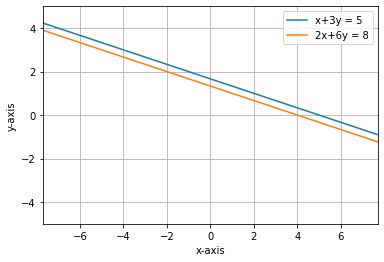
\includegraphics[width=\columnwidth]{assignment2.png}
%\caption{Plot showing the given two lines are parallel}
%\label{Fig 0}
%\end{figure}
